\documentclass{article}
\usepackage[utf8]{inputenc}
\usepackage{xcolor}
\usepackage{multicol}
\usepackage{geometry}
\usepackage{tikz}
\usepackage{pgfplots}
\usepackage{enumitem}
\usepackage{amsmath}
\usepackage{ragged2e}

\geometry{landscape, margin=24pt, paperwidth = 100mm, paperheight = 350mm}

\setlength{\columnsep}{1cm}
\setlength{\columnseprule}{0.2pt}
\renewcommand{\columnseprulecolor}{\color{white}}

\pagecolor[HTML]{2f4f4f}

\pagenumbering{gobble}

\pgfplotsset{compat = 1.15}

\def \listSpacing {28pt}

\begin{document}
\color{white}
\large

{\Large \noindent \textbf{Week 2}}

    \begin{multicols}{3}

    \noindent
    \begin{flushleft}
        Paenitet me quod tu me rogas? Oh, sic, qui stultus plastic continentis rogavi te ut emas. Vides non manducare acidum hydrofluoric per plastic. Erit autem dissolvere metalli petram, vitrum, tellus. Ita quod illic '. Quam de aliquo cum aliqua interdum, maybe? Aliquid viride, huh? Quam vos sunt etiam vivere?
    \end{flushleft}

    \columnbreak
        \centering
        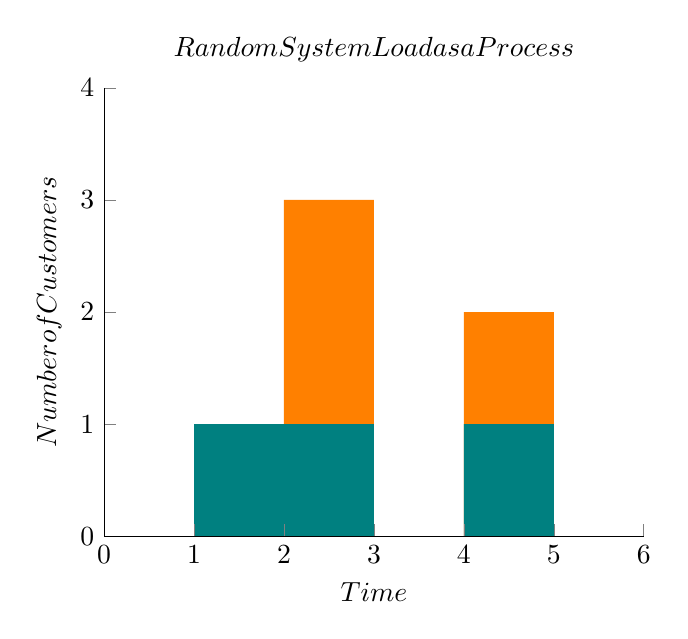
\begin{tikzpicture}
            \begin{axis}[
                axis x line*=bottom,
                axis y line*=left,
                const plot,
                stack plots=y,
                title = $Random System Load as a Process$,
                xlabel = $Time$,
                ylabel = $Number of Customers$,
                ymin = 0,
                xmin = 0,
                ymax = 4,
                xmax = 6,
                enlarge y limits={abs=0},
                area style]

                \addplot[fill=teal,draw opacity=0] coordinates{(0,0) (1,1) (2,1) (3,0) (4,1) (5,1)}\closedcycle;
                \addplot[fill=orange,draw opacity=0] coordinates{(0,0) (1,0) (2,2) (3,0) (4,1) (5,1)}\closedcycle;
            \end{axis}
        \end{tikzpicture}

    \columnbreak

        \begin{enumerate}[label=\arabic*)]
            \setlength\itemsep{\listSpacing}
            \item \quad $ \frac{14}{8} = L^{-}_{sys} \quad [\frac{jobs \cdot time}{time} = jobs]$
            \item \quad $ \frac{11}{8} = L^{-}_{q} \quad [\frac{jobs \cdot time}{time} = jobs]$
            \item \quad $ \frac{3}{8} = L^{-}_{srv} \quad [\frac{jobs \cdot time}{time} = jobs]$
         \end{enumerate}

        \vspace*{\listSpacing}
        \boxed{L^{-}_{sys} = L^{-}_{q} + L^{-}_{srv}}
    \end{multicols}

\end{document}